\documentclass{article}

\usepackage{graphicx}
\usepackage{amsmath}
\usepackage{graphicx}
\graphicspath{{images/}}

\title{APG4011F Assignment 3}
\date{07/05/2015}
\author{Jason David Russell - RSSJAS005}

\begin{document}

\maketitle
\pagenumbering{gobble}

\newpage
\tableofcontents
\pagenumbering{arabic}

\newpage
\section{Introduction}
The purpose of this assignment is to gain an understanding into the principles of image restitution and bundle adjustment.
A python program will be used to demonstrate and simulate how image restitution and bundle adjustment is performed.
The main tasks of this assignment involve creating appropriate fictitious data so that an image ray intersection, resection
and multiple bundle adjustment can be performed. Thereafter, the actual intersection, resection and bundle adjustment will
be carried out and results will be compared to the original fictitious data.


\section{Background}
Image restitution and bundle adjustment has many applications in various fields such as computer vision and photogrammtery.
The objective of image restitution is to reconstruct image rays and a cameras proposition and orientation in space, as they existed during the moment of photography.
This means that a single image ray will pass through a perspective center, image point, and homologous object point, and so
in order to reconstruct an image ray, various parameters need to be taken into consideration.
Perspective center coordinates, camera tilt/attitude, camera focal length/principle distance, image point coordinate (in the
image coordinate system), and correspond object point coordinate are of primary concern.
The process of reconstructing image rays and camera characteristics can be broken down into two main parts, interior and exterior orientation.
Exterior orientation involves parameters concerning the camera in space, while interior orientation involves parameters of actual image rays in the
image space.

\newpage
\subsection{Interior Orientation}
Interior or Inner orientation is described as the reconstruction of the geometry of th bundle of imaging rays as they existed at the time
of photography. It is defined by: the calibrated principle distance of the camera, the position of the principle point in the image plane,
and the geometric distortion characteristics of the lens system.
In this assignment, fictitious image and object points will be created such that an intersection, resection and full bundle adjustment
can be carried out.

\begin{figure}[h!]
\centering
\caption{Interior Orientation depiction.}
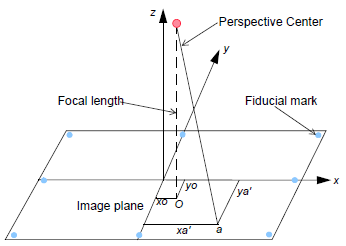
\includegraphics{interior_diagram}
\end{figure}

\begin{figure}[h!]
\centering
\caption{Interior orientation equations.}
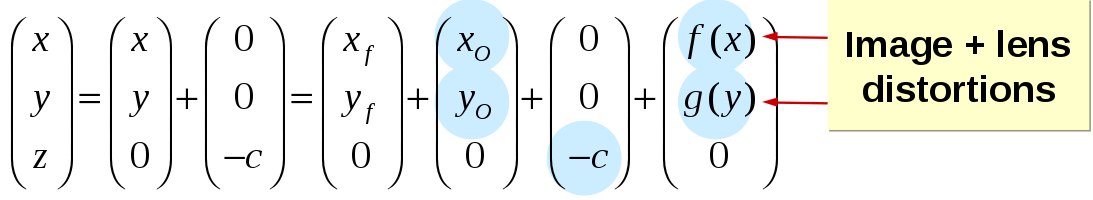
\includegraphics[scale=0.3]{interior_equations}
\end{figure}

\newpage

\subsection{Exterior Orientation}
Exterior or Outer orientation is described as the reconstruction of the position and attitude of the camera as it existed at the time of
photography and is defined by: the position of the projection center, and the rotation angles for each 3D axis.

\begin{figure}[h!]
\centering
\caption{Exterior Orientation depiction.}
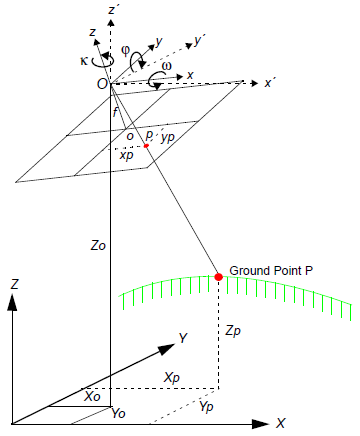
\includegraphics{exterior_diagram}
\end{figure}

\newpage

\subsection{Collinearity Condition}
In order to relate these two systems, the collinearity condition is used and it states that assuming no unmodeled image and lens
distortions, the projection center, object point and corresponding image point should lie on a straight line.

\begin{figure}[h!]
\centering
\caption{Collinearity Condition Equations.}
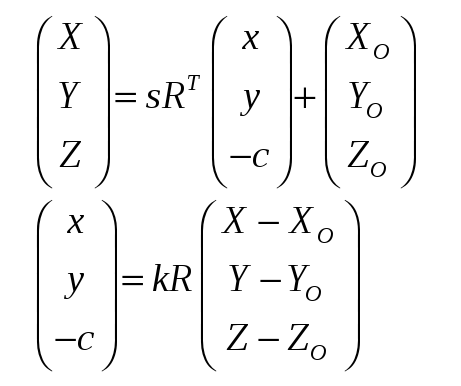
\includegraphics[scale=0.3]{collinearity_equations}
\end{figure}

\newpage

\section{Problem Statement}
There are three main questions which will be addressed in this assignment. They are listed below:

\subsection{Intersection}
Given a set of object points which have homologous points in two separate images, with each image having unique exterior
orientation parameters, set up a least squares adjustment using the collinearity equations to redetermine the object points
from each pair of homologous points from each image. Thereafter, compare the new object coordinates to those original,
generated object coordinates.

\subsection{Resection}
Given a set ob object points, which each have a homologous point in two separate images, set up a least squares adjustment
to determine the exterior orientation parameters of each image,

\subsection{Bundle Adjustment}
Given a set of object points, treat 80\% of them as control, and the remainder as tie points.
Then, use the collinearity equations to set up a least squares adjustment to simultaneously determine the exterior
orientation parameters of the two images as well as the object coordinates of the tie points.

\newpage

\section{Method}
A python program was created which was used to run the various adjustments and calculations pertaining to the questions
in this assignment. Methods are explained in detail below.

\subsection{Creating fictitious Object Points}
Fictitious data needed to be created for the task, this was done using python code.
In order to create fictitious object points, each with two homologous points in different images,
two camera positions were created, each with a unique perspective center.
Parameters for the first image were set up and thirty random points where generated in the first images' image coordinate system.
These random points were then projected down into the object coordinate system using the collinearity equations with
predefined rotations and scales. Then, in order to create the homologous points in the second image, the object points were
reprojected back up to the second image, again using the collinearity equations.
This resulted in three sets of homologous points, those in the first images' image system, those in the object system,
and those in the second images' image system.

\subsection{Intersection}
The intersection in the context of image restitution and bundle adjustment, requires two perspective centers (two images),
each which contain the same object point in them.
This allows for two imaging rays to be constructed and intersected which allows for the determination of the intersection points coordinates.
An imaging ray passes through a perspective center, image point, and object point once interior and exterior orientation has taken place.
Given that three sets of perfectly homologous points had been created, small random errors where added to the second images' image points
to allow for a meaningful comparison of the results of the intersected object points to the existing object points.

\begin{figure}[h!]
\centering
\caption{Intersection.}
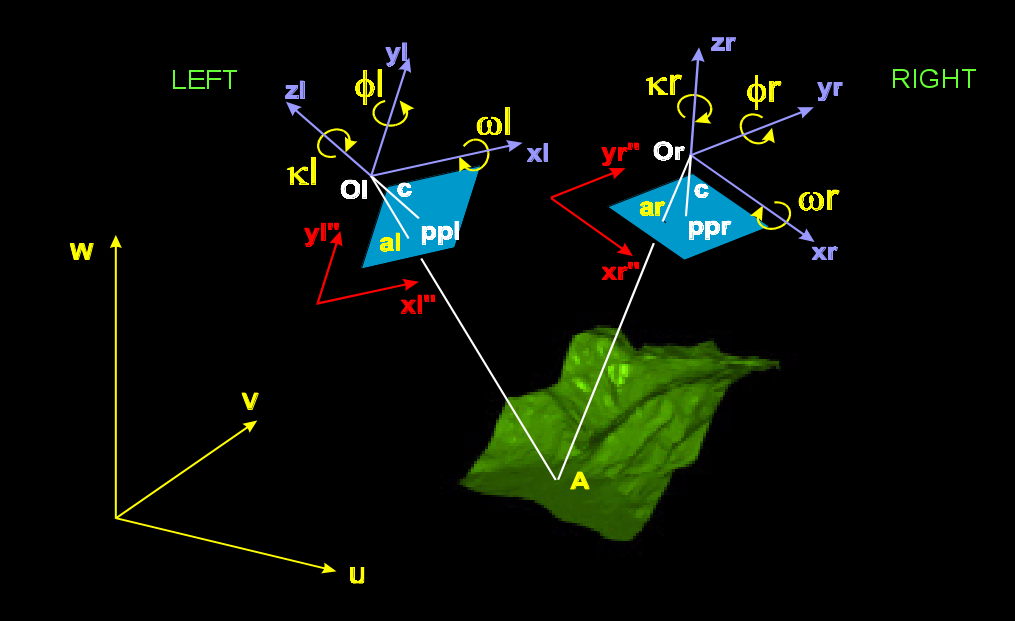
\includegraphics[scale=0.2]{intersection}
\end{figure}


\subsection{Resection}
Using the generated object coordinates as well as the two sets of homologous image coordinates
it is possible to determine the exterior orientation parameters of each image, namely the three rotations
x, y, z and the perspective center coordinates for each image in the object coordinate system. 

\section{Results}

\begin{figure}[h!]
	\centering
	\caption{Simulation.}
	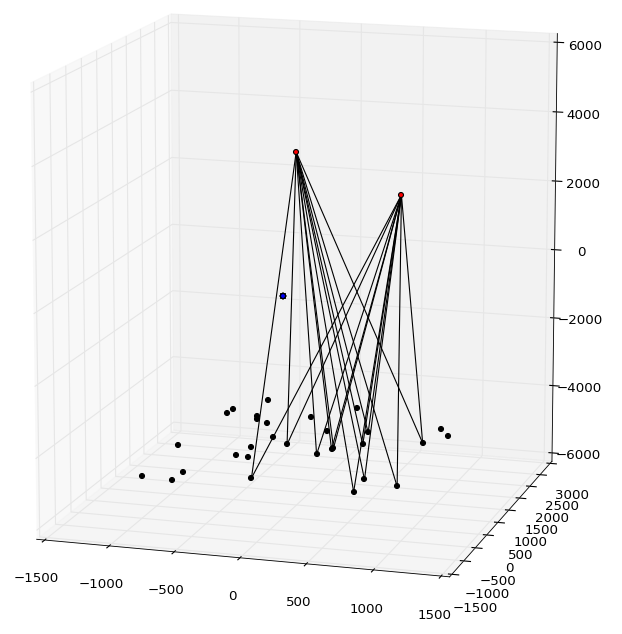
\includegraphics[scale=0.3]{vectors}
\end{figure}
In figure 6, the image ray vectors are visible and run from the two perspective centers to the homologous ground points.


\section{Discussion}

\section{Conclusion}

\end{document}
